% Options for packages loaded elsewhere
\PassOptionsToPackage{unicode}{hyperref}
\PassOptionsToPackage{hyphens}{url}
%
\documentclass[
]{article}
\usepackage{amsmath,amssymb}
\usepackage{lmodern}
\usepackage{iftex}
\ifPDFTeX
  \usepackage[T1]{fontenc}
  \usepackage[utf8]{inputenc}
  \usepackage{textcomp} % provide euro and other symbols
\else % if luatex or xetex
  \usepackage{unicode-math}
  \defaultfontfeatures{Scale=MatchLowercase}
  \defaultfontfeatures[\rmfamily]{Ligatures=TeX,Scale=1}
\fi
% Use upquote if available, for straight quotes in verbatim environments
\IfFileExists{upquote.sty}{\usepackage{upquote}}{}
\IfFileExists{microtype.sty}{% use microtype if available
  \usepackage[]{microtype}
  \UseMicrotypeSet[protrusion]{basicmath} % disable protrusion for tt fonts
}{}
\makeatletter
\@ifundefined{KOMAClassName}{% if non-KOMA class
  \IfFileExists{parskip.sty}{%
    \usepackage{parskip}
  }{% else
    \setlength{\parindent}{0pt}
    \setlength{\parskip}{6pt plus 2pt minus 1pt}}
}{% if KOMA class
  \KOMAoptions{parskip=half}}
\makeatother
\usepackage{xcolor}
\IfFileExists{xurl.sty}{\usepackage{xurl}}{} % add URL line breaks if available
\IfFileExists{bookmark.sty}{\usepackage{bookmark}}{\usepackage{hyperref}}
\hypersetup{
  pdftitle={Estimating Systematic Risk Using the Capital Asset Pricing Model (CAPM)},
  pdfauthor={Eldar Gasimov},
  hidelinks,
  pdfcreator={LaTeX via pandoc}}
\urlstyle{same} % disable monospaced font for URLs
\usepackage[margin=1in]{geometry}
\usepackage{color}
\usepackage{fancyvrb}
\newcommand{\VerbBar}{|}
\newcommand{\VERB}{\Verb[commandchars=\\\{\}]}
\DefineVerbatimEnvironment{Highlighting}{Verbatim}{commandchars=\\\{\}}
% Add ',fontsize=\small' for more characters per line
\usepackage{framed}
\definecolor{shadecolor}{RGB}{248,248,248}
\newenvironment{Shaded}{\begin{snugshade}}{\end{snugshade}}
\newcommand{\AlertTok}[1]{\textcolor[rgb]{0.94,0.16,0.16}{#1}}
\newcommand{\AnnotationTok}[1]{\textcolor[rgb]{0.56,0.35,0.01}{\textbf{\textit{#1}}}}
\newcommand{\AttributeTok}[1]{\textcolor[rgb]{0.77,0.63,0.00}{#1}}
\newcommand{\BaseNTok}[1]{\textcolor[rgb]{0.00,0.00,0.81}{#1}}
\newcommand{\BuiltInTok}[1]{#1}
\newcommand{\CharTok}[1]{\textcolor[rgb]{0.31,0.60,0.02}{#1}}
\newcommand{\CommentTok}[1]{\textcolor[rgb]{0.56,0.35,0.01}{\textit{#1}}}
\newcommand{\CommentVarTok}[1]{\textcolor[rgb]{0.56,0.35,0.01}{\textbf{\textit{#1}}}}
\newcommand{\ConstantTok}[1]{\textcolor[rgb]{0.00,0.00,0.00}{#1}}
\newcommand{\ControlFlowTok}[1]{\textcolor[rgb]{0.13,0.29,0.53}{\textbf{#1}}}
\newcommand{\DataTypeTok}[1]{\textcolor[rgb]{0.13,0.29,0.53}{#1}}
\newcommand{\DecValTok}[1]{\textcolor[rgb]{0.00,0.00,0.81}{#1}}
\newcommand{\DocumentationTok}[1]{\textcolor[rgb]{0.56,0.35,0.01}{\textbf{\textit{#1}}}}
\newcommand{\ErrorTok}[1]{\textcolor[rgb]{0.64,0.00,0.00}{\textbf{#1}}}
\newcommand{\ExtensionTok}[1]{#1}
\newcommand{\FloatTok}[1]{\textcolor[rgb]{0.00,0.00,0.81}{#1}}
\newcommand{\FunctionTok}[1]{\textcolor[rgb]{0.00,0.00,0.00}{#1}}
\newcommand{\ImportTok}[1]{#1}
\newcommand{\InformationTok}[1]{\textcolor[rgb]{0.56,0.35,0.01}{\textbf{\textit{#1}}}}
\newcommand{\KeywordTok}[1]{\textcolor[rgb]{0.13,0.29,0.53}{\textbf{#1}}}
\newcommand{\NormalTok}[1]{#1}
\newcommand{\OperatorTok}[1]{\textcolor[rgb]{0.81,0.36,0.00}{\textbf{#1}}}
\newcommand{\OtherTok}[1]{\textcolor[rgb]{0.56,0.35,0.01}{#1}}
\newcommand{\PreprocessorTok}[1]{\textcolor[rgb]{0.56,0.35,0.01}{\textit{#1}}}
\newcommand{\RegionMarkerTok}[1]{#1}
\newcommand{\SpecialCharTok}[1]{\textcolor[rgb]{0.00,0.00,0.00}{#1}}
\newcommand{\SpecialStringTok}[1]{\textcolor[rgb]{0.31,0.60,0.02}{#1}}
\newcommand{\StringTok}[1]{\textcolor[rgb]{0.31,0.60,0.02}{#1}}
\newcommand{\VariableTok}[1]{\textcolor[rgb]{0.00,0.00,0.00}{#1}}
\newcommand{\VerbatimStringTok}[1]{\textcolor[rgb]{0.31,0.60,0.02}{#1}}
\newcommand{\WarningTok}[1]{\textcolor[rgb]{0.56,0.35,0.01}{\textbf{\textit{#1}}}}
\usepackage{graphicx}
\makeatletter
\def\maxwidth{\ifdim\Gin@nat@width>\linewidth\linewidth\else\Gin@nat@width\fi}
\def\maxheight{\ifdim\Gin@nat@height>\textheight\textheight\else\Gin@nat@height\fi}
\makeatother
% Scale images if necessary, so that they will not overflow the page
% margins by default, and it is still possible to overwrite the defaults
% using explicit options in \includegraphics[width, height, ...]{}
\setkeys{Gin}{width=\maxwidth,height=\maxheight,keepaspectratio}
% Set default figure placement to htbp
\makeatletter
\def\fps@figure{htbp}
\makeatother
\setlength{\emergencystretch}{3em} % prevent overfull lines
\providecommand{\tightlist}{%
  \setlength{\itemsep}{0pt}\setlength{\parskip}{0pt}}
\setcounter{secnumdepth}{-\maxdimen} % remove section numbering
\usepackage{pdflscape}
\newcommand{\blandscape}{\begin{landscape}}
\newcommand{\elandscape}{\end{landscape}}
\usepackage{booktabs}
\usepackage{longtable}
\usepackage{array}
\usepackage{multirow}
\usepackage{wrapfig}
\usepackage{float}
\usepackage{colortbl}
\usepackage{pdflscape}
\usepackage{tabu}
\usepackage{threeparttable}
\usepackage{threeparttablex}
\usepackage[normalem]{ulem}
\usepackage{makecell}
\usepackage{xcolor}
\ifLuaTeX
  \usepackage{selnolig}  % disable illegal ligatures
\fi

\title{\textbf{Estimating Systematic Risk Using the Capital Asset
Pricing Model (CAPM)}}
\usepackage{etoolbox}
\makeatletter
\providecommand{\subtitle}[1]{% add subtitle to \maketitle
  \apptocmd{\@title}{\par {\large #1 \par}}{}{}
}
\makeatother
\subtitle{\textbf{\emph{Applying CAPM to IBM and Microsoft Stocks,
2002-2007}}}
\author{Eldar Gasimov}
\date{Wednesday October 26, 2022}

\begin{document}
\maketitle

{
\setcounter{tocdepth}{3}
\tableofcontents
}
\newpage

\hypertarget{summary}{%
\section{Summary}\label{summary}}

\begin{itemize}
\tightlist
\item
  The regression equation estimate for GM is
  \(gm_premium = -0.005876 + 1.181982Market Premium\) while that of
  Microsoft is
  \(microsoft_premium = -0.003122 + 0.983402Market Premium\).
\item
  Both Microsoft and GM have a \(\beta\) of that do not differ
  signifcantly from 1.
\item
  This observation means that the returns from these stocks are as
  volatile as the returns of a market portfolio.
\item
  The \(\alpha\) for both stocks is not statistically significant.
\item
  The regressions could suffer from omitted variable bias.
\end{itemize}

\hypertarget{question-a-download-the-data-into-r-and-provide-summary-statistics-for-each-variable.}{%
\section{\texorpdfstring{\textbf{Question A: Download the Data into R
and Provide Summary Statistics for Each
variable.}}{Question A: Download the Data into R and Provide Summary Statistics for Each variable.}}\label{question-a-download-the-data-into-r-and-provide-summary-statistics-for-each-variable.}}

I load the data into R using the following line of code. Table 1
summarises the variables contained in the dataset;

\begin{Shaded}
\begin{Highlighting}[]
\NormalTok{capm\_data }\OtherTok{\textless{}{-}}\NormalTok{ readxl}\SpecialCharTok{::}\FunctionTok{read\_xlsx}\NormalTok{(}\StringTok{"capm.xlsx"}\NormalTok{) }
\end{Highlighting}
\end{Shaded}

\begin{table}[!h]

\caption{\label{tab:unnamed-chunk-2}Variables Description}
\centering
\begin{tabular}[t]{ll}
\toprule
Variable & Description\\
\midrule
Date & The date of data collection.\\
SP500 & S\&P 500 Index at the corresponding date\\
GM & Stock price for General Motors on the correponding date.\\
MICROSOFT & Stock price for Microsoft on the correponding date.\\
USTB3M & US 3 month treasury bills coupon rate.\\
\bottomrule
\end{tabular}
\end{table}

Table 2 below shows the first 6 rows in the data.

\begin{Shaded}
\begin{Highlighting}[]
\FunctionTok{head}\NormalTok{(capm\_data) }\SpecialCharTok{\%\textgreater{}\%} 
    
    \FunctionTok{formatting\_function}\NormalTok{(}\AttributeTok{caption =} \StringTok{"An Overview of the Data"}\NormalTok{)}
\end{Highlighting}
\end{Shaded}

\begin{table}[!h]

\caption{\label{tab:unnamed-chunk-3}An Overview of the Data}
\centering
\begin{tabular}[t]{lrrrr}
\toprule
Date & SP500 & GM & MICROSOFT & USTB3M\\
\midrule
2002-01-01 & 1130.20 & 39.55 & 27.33 & 1.73\\
2002-02-01 & 1106.73 & 41.40 & 25.02 & 1.75\\
2002-03-01 & 1147.39 & 47.23 & 25.87 & 1.77\\
2002-04-01 & 1076.92 & 50.12 & 22.41 & 1.78\\
2002-05-01 & 1067.14 & 48.92 & 21.84 & 1.77\\
\addlinespace
2002-06-01 & 989.82 & 42.07 & 23.46 & 1.75\\
\bottomrule
\end{tabular}
\end{table}

\begin{Shaded}
\begin{Highlighting}[]
\NormalTok{capm\_data }\OtherTok{\textless{}{-}}\NormalTok{ capm\_data }\SpecialCharTok{\%\textgreater{}\%} 
    
    \FunctionTok{clean\_names}\NormalTok{()}
\end{Highlighting}
\end{Shaded}

\hypertarget{exploring-the-data}{%
\subsection{\texorpdfstring{\textbf{\emph{Exploring the
Data}}}{Exploring the Data}}\label{exploring-the-data}}

I start by plotting the data trends from 2002 and then summarise the
data.

\newpage
\begin{landscape}

\begin{Shaded}
\begin{Highlighting}[]
\NormalTok{capm\_data }\SpecialCharTok{\%\textgreater{}\%} 
    \FunctionTok{pivot\_longer}\NormalTok{(}\SpecialCharTok{{-}}\NormalTok{date, }\AttributeTok{names\_to =} \StringTok{"stock"}\NormalTok{, }\AttributeTok{values\_to =} \StringTok{"price"}\NormalTok{) }\SpecialCharTok{\%\textgreater{}\%} 
    \FunctionTok{ggplot}\NormalTok{(}\AttributeTok{mapping =} \FunctionTok{aes}\NormalTok{(}\AttributeTok{x =}\NormalTok{ date, }\AttributeTok{y =}\NormalTok{ price, }\AttributeTok{color =}\NormalTok{ stock)) }\SpecialCharTok{+} 
    \FunctionTok{geom\_line}\NormalTok{() }\SpecialCharTok{+} \FunctionTok{facet\_wrap}\NormalTok{(}\SpecialCharTok{\textasciitilde{}}\NormalTok{stock, }\AttributeTok{scales =} \StringTok{"free\_y"}\NormalTok{) }\SpecialCharTok{+} 
    \FunctionTok{theme\_tq}\NormalTok{() }\SpecialCharTok{+} \FunctionTok{theme}\NormalTok{(}\AttributeTok{legend.position =} \StringTok{"none"}\NormalTok{) }\SpecialCharTok{+} 
    \FunctionTok{labs}\NormalTok{(}\AttributeTok{x =} \StringTok{""}\NormalTok{, }\AttributeTok{y =} \StringTok{""}\NormalTok{, }\AttributeTok{title =} \StringTok{"Trends in GM, Microsoft, S\&P 500, and 90 Days US T{-}Bill Rate, 2002{-}2007"}\NormalTok{, }\AttributeTok{caption =} \StringTok{"Note the different y{-}scales"}\NormalTok{)}
\end{Highlighting}
\end{Shaded}

\begin{figure}
\centering
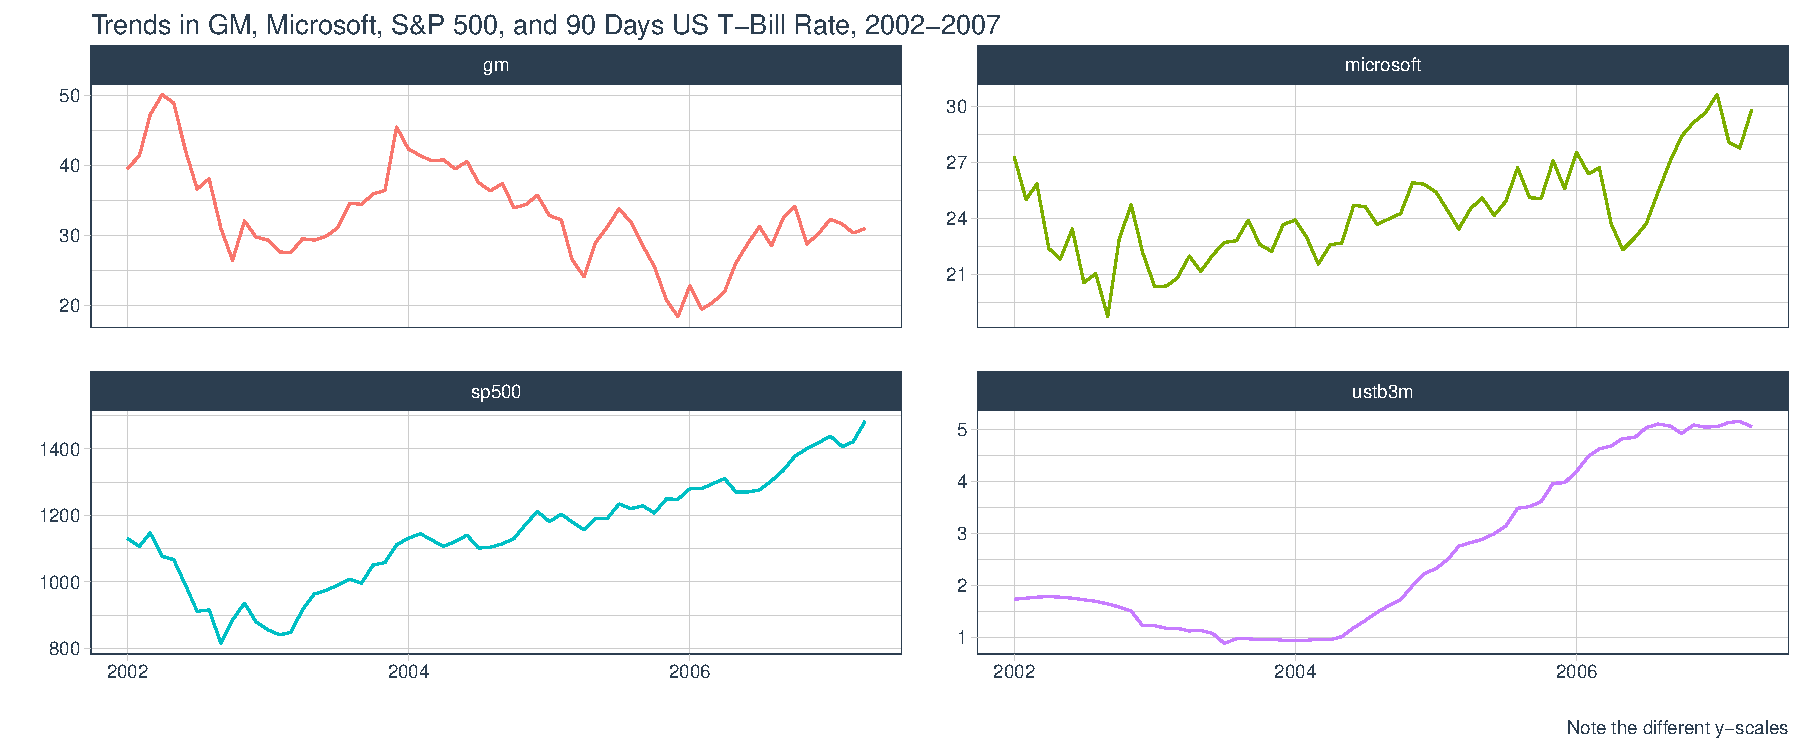
\includegraphics{capm_files/figure-latex/unnamed-chunk-4-1.pdf}
\caption{Trends in GM, Microsoft, S\&P 500, and 90 Days US T-Bill Rate,
2002-2007}
\end{figure}

\end{landscape}
\newpage

\begin{Shaded}
\begin{Highlighting}[]
\NormalTok{capm\_data }\SpecialCharTok{\%\textgreater{}\%} 
    \FunctionTok{select}\NormalTok{(}\SpecialCharTok{{-}}\NormalTok{date) }\SpecialCharTok{\%\textgreater{}\%}\NormalTok{ skimr}\SpecialCharTok{::}\FunctionTok{skim\_without\_charts}\NormalTok{() }\SpecialCharTok{\%\textgreater{}\%}
    \FunctionTok{select}\NormalTok{(}\SpecialCharTok{{-}}\NormalTok{skim\_type, }\SpecialCharTok{{-}}\NormalTok{complete\_rate) }\SpecialCharTok{\%\textgreater{}\%} 
    \FunctionTok{rename}\NormalTok{(}\AttributeTok{Variable =}\NormalTok{ skim\_variable, }\AttributeTok{Missing =}\NormalTok{ n\_missing, }
           \AttributeTok{Mean =}\NormalTok{ numeric.mean, }\AttributeTok{SD =}\NormalTok{ numeric.sd, }\AttributeTok{Min =}\NormalTok{ numeric.p0, }
           \AttributeTok{Q1 =}\NormalTok{ numeric.p25, }\AttributeTok{Median =}\NormalTok{ numeric.p50, }
           \AttributeTok{Q3 =}\NormalTok{ numeric.p75, }\AttributeTok{Max =}\NormalTok{ numeric.p100) }\SpecialCharTok{\%\textgreater{}\%} 
    \FunctionTok{formatting\_function}\NormalTok{(}\AttributeTok{caption =} \StringTok{"Descriptive Statistics"}\NormalTok{) }\SpecialCharTok{\%\textgreater{}\%} 
    \FunctionTok{footnote}\NormalTok{(}\AttributeTok{number =} \FunctionTok{c}\NormalTok{(}\StringTok{"sp500: S\&P 500 Index."}\NormalTok{, }\StringTok{"gm: General Motors Stock Pirces."}\NormalTok{, }\StringTok{"microsoft: MicroSoft Stock Prices."}\NormalTok{, }\StringTok{"ustb3m: US 3 month Treasury bills."}\NormalTok{))}
\end{Highlighting}
\end{Shaded}

\begin{table}[!h]

\caption{\label{tab:unnamed-chunk-5}Descriptive Statistics}
\centering
\begin{tabular}[t]{lrrrrrrrr}
\toprule
Variable & Missing & Mean & SD & Min & Q1 & Median & Q3 & Max\\
\midrule
sp500 & 0 & 1142.922500 & 164.177365 & 815.28 & 1040.0350 & 1142.89 & 1254.632 & 1482.37\\
gm & 0 & 32.831562 & 6.945924 & 18.44 & 28.8725 & 31.98 & 36.835 & 50.12\\
microsoft & 0 & 24.362188 & 2.527132 & 18.76 & 22.6175 & 24.09 & 25.855 & 30.65\\
ustb3m & 0 & 2.577031 & 1.557040 & 0.88 & 1.1775 & 1.77 & 4.025 & 5.15\\
\bottomrule
\multicolumn{9}{l}{\rule{0pt}{1em}\textsuperscript{1} sp500: S\&P 500 Index.}\\
\multicolumn{9}{l}{\rule{0pt}{1em}\textsuperscript{2} gm: General Motors Stock Pirces.}\\
\multicolumn{9}{l}{\rule{0pt}{1em}\textsuperscript{3} microsoft: MicroSoft Stock Prices.}\\
\multicolumn{9}{l}{\rule{0pt}{1em}\textsuperscript{4} ustb3m: US 3 month Treasury bills.}\\
\end{tabular}
\end{table}

\hypertarget{question-b-computing-the-returns-excess-returns-of-market-and-each-of-the-companies-over-the-risk-free-rate.}{%
\section{\texorpdfstring{\textbf{Question B: Computing the Returns,
Excess Returns of market and each of the companies over the risk free
rate.}}{Question B: Computing the Returns, Excess Returns of market and each of the companies over the risk free rate.}}\label{question-b-computing-the-returns-excess-returns-of-market-and-each-of-the-companies-over-the-risk-free-rate.}}

\hypertarget{returns}{%
\subsection{\texorpdfstring{\textbf{\emph{Returns}}}{Returns}}\label{returns}}

We compute the log returns for the market (S\&P500), Microsoft, and GM.

\begin{Shaded}
\begin{Highlighting}[]
\NormalTok{returns }\OtherTok{\textless{}{-}}\NormalTok{ capm\_data }\SpecialCharTok{\%\textgreater{}\%} 
    \FunctionTok{summarise}\NormalTok{(}\AttributeTok{rgm =} \FunctionTok{diff}\NormalTok{(}\FunctionTok{log}\NormalTok{(gm), }\AttributeTok{lag =} \DecValTok{1}\NormalTok{),}
              
              \AttributeTok{rmt =} \FunctionTok{diff}\NormalTok{(}\FunctionTok{log}\NormalTok{(microsoft), }\AttributeTok{lag =} \DecValTok{1}\NormalTok{),}
              
              \AttributeTok{rm =} \FunctionTok{diff}\NormalTok{(}\FunctionTok{log}\NormalTok{(sp500), }\AttributeTok{lag =} \DecValTok{1}\NormalTok{),}
              
              \AttributeTok{rf =} \FunctionTok{diff}\NormalTok{(}\FunctionTok{log}\NormalTok{(ustb3m), }\AttributeTok{lag =} \DecValTok{1}\NormalTok{)) }

\FunctionTok{head}\NormalTok{(returns) }\SpecialCharTok{\%\textgreater{}\%} 
    \FunctionTok{formatting\_function}\NormalTok{(}\AttributeTok{caption =}  \StringTok{"Overview of Returns"}\NormalTok{)}
\end{Highlighting}
\end{Shaded}

\begin{table}[!h]

\caption{\label{tab:unnamed-chunk-6}Overview of Returns}
\centering
\begin{tabular}[t]{rrrr}
\toprule
rgm & rmt & rm & rf\\
\midrule
0.0457152 & -0.0883095 & -0.0209849 & 0.0114944\\
0.1317484 & 0.0334085 & 0.0360801 & 0.0113638\\
0.0593908 & -0.1435767 & -0.0633847 & 0.0056338\\
-0.0242338 & -0.0257641 & -0.0091229 & -0.0056338\\
-0.1508514 & 0.0715537 & -0.0752143 & -0.0113638\\
\addlinespace
-0.1381944 & -0.1309771 & -0.0822999 & -0.0172915\\
\bottomrule
\end{tabular}
\end{table}

\hypertarget{excess-returns-of-the-market-and-each-of-the-companies-and-the-capm-model}{%
\subsection{\texorpdfstring{\textbf{\emph{Excess Returns of the Market
and Each of the companies and the CAPM
Model}}}{Excess Returns of the Market and Each of the companies and the CAPM Model}}\label{excess-returns-of-the-market-and-each-of-the-companies-and-the-capm-model}}

The CAPM model is as follows (Bodie, Z., et al, 2018):

\(r_{s} - r_{f} = \alpha + \beta (r_{m} - r_{f})\)

The left hand side consists of the difference beteen the returns of
stock s and the risk free rate proxied by the US 3 month treasury bill
rate. \(\alpha\) and \(\beta\) are the coefficients of the equation that
e estimate in this exercise. The term \(r_{m} - r_{f}\) is the market
risk premium computed as the return of the market portfolio less the
risk free rate.

This section starts by computing the market premium, defined as the
return of the market (S\&P) index less the risk free rate.

\(market premium = rm - rf\)

Next, from the returns of each of the stocks (GM - rgm and Microsoft-
rmt), we subtract the risk free rate (rf) to get the Microsoft premium
(mt\_premium) and the General Motors premium (gm\_premium).

\(mt_premium = rmt - rf\)

\(gm_premium = rgm - rf\)

\begin{Shaded}
\begin{Highlighting}[]
\NormalTok{regression\_data }\OtherTok{\textless{}{-}}\NormalTok{ returns }\SpecialCharTok{\%\textgreater{}\%} 
    \FunctionTok{transmute}\NormalTok{(}\AttributeTok{market\_premium =}\NormalTok{ rm }\SpecialCharTok{{-}}\NormalTok{ rf,}
           \AttributeTok{microsoft\_premium =}\NormalTok{ rmt }\SpecialCharTok{{-}}\NormalTok{ rf,}
           \AttributeTok{gm\_premium =}\NormalTok{ rgm }\SpecialCharTok{{-}}\NormalTok{ rf)}

\FunctionTok{head}\NormalTok{(regression\_data) }\SpecialCharTok{\%\textgreater{}\%} 
    \FunctionTok{formatting\_function}\NormalTok{(}\AttributeTok{caption =} \StringTok{"Sample Data for Regression Analysis"}\NormalTok{)}
\end{Highlighting}
\end{Shaded}

\begin{table}[!h]

\caption{\label{tab:unnamed-chunk-7}Sample Data for Regression Analysis}
\centering
\begin{tabular}[t]{rrr}
\toprule
market\_premium & microsoft\_premium & gm\_premium\\
\midrule
-0.0324793 & -0.0998039 & 0.0342208\\
0.0247163 & 0.0220447 & 0.1203846\\
-0.0690185 & -0.1492105 & 0.0537570\\
-0.0034891 & -0.0201303 & -0.0186000\\
-0.0638506 & 0.0829175 & -0.1394877\\
\addlinespace
-0.0650084 & -0.1136856 & -0.1209029\\
\bottomrule
\end{tabular}
\end{table}

\hypertarget{question-c-regression-analysis-of-the-capm-equations}{%
\section{\texorpdfstring{\textbf{Question C: Regression Analysis of the
CAPM
equations}}{Question C: Regression Analysis of the CAPM equations}}\label{question-c-regression-analysis-of-the-capm-equations}}

The regression analysis for GM stock and Microsoft stock are as follows.

\hypertarget{gm-stock}{%
\subsection{\texorpdfstring{\textbf{\emph{GM
stock}}}{GM stock}}\label{gm-stock}}

\begin{Shaded}
\begin{Highlighting}[]
\NormalTok{gm\_regression }\OtherTok{\textless{}{-}} \FunctionTok{lm}\NormalTok{(gm\_premium }\SpecialCharTok{\textasciitilde{}}\NormalTok{ market\_premium, }\AttributeTok{data =}\NormalTok{ regression\_data)}

\FunctionTok{summary}\NormalTok{(gm\_regression)}
\end{Highlighting}
\end{Shaded}

\begin{verbatim}
## 
## Call:
## lm(formula = gm_premium ~ market_premium, data = regression_data)
## 
## Residuals:
##       Min        1Q    Median        3Q       Max 
## -0.255539 -0.042951 -0.007383  0.048576  0.220929 
## 
## Coefficients:
##                 Estimate Std. Error t value Pr(>|t|)    
## (Intercept)    -0.005876   0.012054  -0.487    0.628    
## market_premium  1.181982   0.174126   6.788 5.35e-09 ***
## ---
## Signif. codes:  0 '***' 0.001 '**' 0.01 '*' 0.05 '.' 0.1 ' ' 1
## 
## Residual standard error: 0.09405 on 61 degrees of freedom
## Multiple R-squared:  0.4303, Adjusted R-squared:  0.421 
## F-statistic: 46.08 on 1 and 61 DF,  p-value: 5.353e-09
\end{verbatim}

\hypertarget{microsoft-stock}{%
\subsection{\texorpdfstring{\textbf{\emph{MicroSoft
Stock}}}{MicroSoft Stock}}\label{microsoft-stock}}

\begin{Shaded}
\begin{Highlighting}[]
\NormalTok{microsoft\_regression }\OtherTok{\textless{}{-}} \FunctionTok{lm}\NormalTok{(microsoft\_premium }\SpecialCharTok{\textasciitilde{}}\NormalTok{ market\_premium, }\AttributeTok{data=}\NormalTok{ regression\_data)}

\FunctionTok{summary}\NormalTok{(microsoft\_regression)}
\end{Highlighting}
\end{Shaded}

\begin{verbatim}
## 
## Call:
## lm(formula = microsoft_premium ~ market_premium, data = regression_data)
## 
## Residuals:
##       Min        1Q    Median        3Q       Max 
## -0.128021 -0.037924  0.003073  0.029409  0.148830 
## 
## Coefficients:
##                 Estimate Std. Error t value Pr(>|t|)    
## (Intercept)    -0.003122   0.006558  -0.476    0.636    
## market_premium  0.983402   0.094735  10.381 4.19e-15 ***
## ---
## Signif. codes:  0 '***' 0.001 '**' 0.01 '*' 0.05 '.' 0.1 ' ' 1
## 
## Residual standard error: 0.05117 on 61 degrees of freedom
## Multiple R-squared:  0.6385, Adjusted R-squared:  0.6326 
## F-statistic: 107.8 on 1 and 61 DF,  p-value: 4.191e-15
\end{verbatim}

\hypertarget{question-d-interpreting-the-results-of-the-regression}{%
\section{\texorpdfstring{\textbf{Question D: Interpreting the Results of
the
Regression}}{Question D: Interpreting the Results of the Regression}}\label{question-d-interpreting-the-results-of-the-regression}}

The coefficient for the GM stock (\(\beta\)) is 1.181982. This means
that GM stock is riskier than the market. Specifically, when the market
risk premium rises by 1 unit, the risk premium for the GM stock
increases by 1.181982, ceteris paribus. Put another ay, the GM stock is
more volatile or riskier than the market given it has a \(\beta > 1\).
Hence, the inclusion of the GM stock to a market portfolio will raise
its risk.

The coefficient for the Microsoft stock (\(\beta\)) is 0.983402. This
means that Microsoft stock is marginally less riskier than the market.
Specifically, when the market risk premium rises by 1 unit, the risk
premium for the Microsoft stock increases by 0.983402 units all else
remaining constant. Put another way, the Microsoft stock is marginally
less volatile or less riskier than the market portfolio given it has a
\(\beta < 1\). Hence, the inclusion of the Microsoft stock to a market
portfolio will marginally lower its risk.

\hypertarget{question-e-hypothesis-testing-beta-1-at-5-level-of-confidence}{%
\section{\texorpdfstring{\textbf{Question E: Hypothesis Testing
\(\beta = 1\) at 5\% Level of
Confidence}}{Question E: Hypothesis Testing \textbackslash beta = 1 at 5\% Level of Confidence}}\label{question-e-hypothesis-testing-beta-1-at-5-level-of-confidence}}

\hypertarget{gm-stock-1}{%
\subsection{\texorpdfstring{\textbf{\emph{GM
stock}}}{GM stock}}\label{gm-stock-1}}

In this case, e test the following hypothesis.

Ho: \(\beta = 1\) HA: \(\beta \neq 1\)

Note that this is two sided test. We compute the t-statistic. Note that
e draw the figures from the regression output- the coefficient
(\(\beta\)), standard error and degrees of freedom. We conclude that
\(\beta = 1\) given that 0.8499535 \textgreater{} 0.05.

\(t-stat = \frac{(\beta - hypothesized_Beta)}{se(\beta)}\)

\begin{Shaded}
\begin{Highlighting}[]
\NormalTok{t\_stat\_gm }\OtherTok{=}\NormalTok{ (}\FloatTok{1.181982} \SpecialCharTok{{-}} \DecValTok{1}\NormalTok{) }\SpecialCharTok{/} \FloatTok{0.174126}
\NormalTok{t\_stat\_gm}
\end{Highlighting}
\end{Shaded}

\begin{verbatim}
## [1] 1.045117
\end{verbatim}

\begin{Shaded}
\begin{Highlighting}[]
\FunctionTok{pt}\NormalTok{(t\_stat\_gm, }\AttributeTok{df =} \DecValTok{61}\NormalTok{)}
\end{Highlighting}
\end{Shaded}

\begin{verbatim}
## [1] 0.8499535
\end{verbatim}

\hypertarget{microsoft-stock-1}{%
\subsection{\texorpdfstring{\textbf{Microsoft
Stock}}{Microsoft Stock}}\label{microsoft-stock-1}}

We repeat the same exercise for Microsoft and again fail to reject the
NULL hypothesis. We conclude that \(\beta = 1\) because 0.4307496
\textgreater{} 0.05.

\begin{Shaded}
\begin{Highlighting}[]
\NormalTok{t\_stat\_microsoft }\OtherTok{=}\NormalTok{ (}\FloatTok{0.983402} \SpecialCharTok{{-}} \DecValTok{1}\NormalTok{) }\SpecialCharTok{/} \FloatTok{0.094735}
\NormalTok{t\_stat\_microsoft}
\end{Highlighting}
\end{Shaded}

\begin{verbatim}
## [1] -0.1752045
\end{verbatim}

\begin{Shaded}
\begin{Highlighting}[]
\FunctionTok{pt}\NormalTok{(t\_stat\_microsoft, }\AttributeTok{df =} \DecValTok{61}\NormalTok{)}
\end{Highlighting}
\end{Shaded}

\begin{verbatim}
## [1] 0.4307496
\end{verbatim}

\hypertarget{question-f-95-confidence-interval-for-the-variance}{%
\section{\texorpdfstring{\textbf{Question F: 95\% Confidence Interval
for the
Variance}}{Question F: 95\% Confidence Interval for the Variance}}\label{question-f-95-confidence-interval-for-the-variance}}

In this section, we compute a 95\% confidence interval for the variance
or volatility of both stocks. Given a random sample with sample variance
\(S^{2}\), estimating the population variance follos from the equation
below.

\(Q = \frac{(n - 1)S^{2}}{\sigma^{2}} ~ Chisq(df = n - 1)\)

Thus, the 95\% confidence interval is:

\hypertarget{gm-stock-2}{%
\subsection{\texorpdfstring{\textbf{\emph{GM
Stock}}}{GM Stock}}\label{gm-stock-2}}

\begin{Shaded}
\begin{Highlighting}[]
\NormalTok{gm\_var }\OtherTok{=} \FunctionTok{var}\NormalTok{(regression\_data}\SpecialCharTok{$}\NormalTok{gm\_premium)}

\NormalTok{n }\OtherTok{=} \FunctionTok{nrow}\NormalTok{(regression\_data)}

\NormalTok{((n }\SpecialCharTok{{-}} \DecValTok{1}\NormalTok{) }\SpecialCharTok{*}\NormalTok{ gm\_var) }\SpecialCharTok{/} \FunctionTok{qchisq}\NormalTok{(}\FunctionTok{c}\NormalTok{(}\FloatTok{0.975}\NormalTok{, }\FloatTok{0.05}\NormalTok{), n }\SpecialCharTok{{-}} \DecValTok{1}\NormalTok{)}
\end{Highlighting}
\end{Shaded}

\begin{verbatim}
## [1] 0.01105827 0.02110053
\end{verbatim}

\hypertarget{microsoft-stock-2}{%
\subsection{\texorpdfstring{\textbf{\emph{Microsoft
Stock}}}{Microsoft Stock}}\label{microsoft-stock-2}}

\begin{Shaded}
\begin{Highlighting}[]
\NormalTok{mt\_var }\OtherTok{\textless{}{-}} \FunctionTok{var}\NormalTok{(regression\_data}\SpecialCharTok{$}\NormalTok{microsoft\_premium)}

\NormalTok{((n }\SpecialCharTok{{-}} \DecValTok{1}\NormalTok{) }\SpecialCharTok{*}\NormalTok{ mt\_var) }\SpecialCharTok{/} \FunctionTok{qchisq}\NormalTok{(}\FunctionTok{c}\NormalTok{(}\FloatTok{0.975}\NormalTok{, }\FloatTok{0.05}\NormalTok{), n }\SpecialCharTok{{-}} \DecValTok{1}\NormalTok{)}
\end{Highlighting}
\end{Shaded}

\begin{verbatim}
## [1] 0.005158699 0.009843427
\end{verbatim}

\hypertarget{checking-the-model-assumptions}{%
\section{\texorpdfstring{\textbf{Checking the model
assumptions}}{Checking the model assumptions}}\label{checking-the-model-assumptions}}

Given that there is only one independent variable, the relevant
assumtions are:

\begin{itemize}
\tightlist
\item
  Linearity
\item
  Homogeneity of variance
\item
  Normality of residuals
\end{itemize}

Overall, both models appear to meet the regression assumptions except
for normality of residuals for the GM stock.

There is possibility of omitted variables bias in the analysis.

\newpage

\begin{landscape}

\begin{figure}
\centering
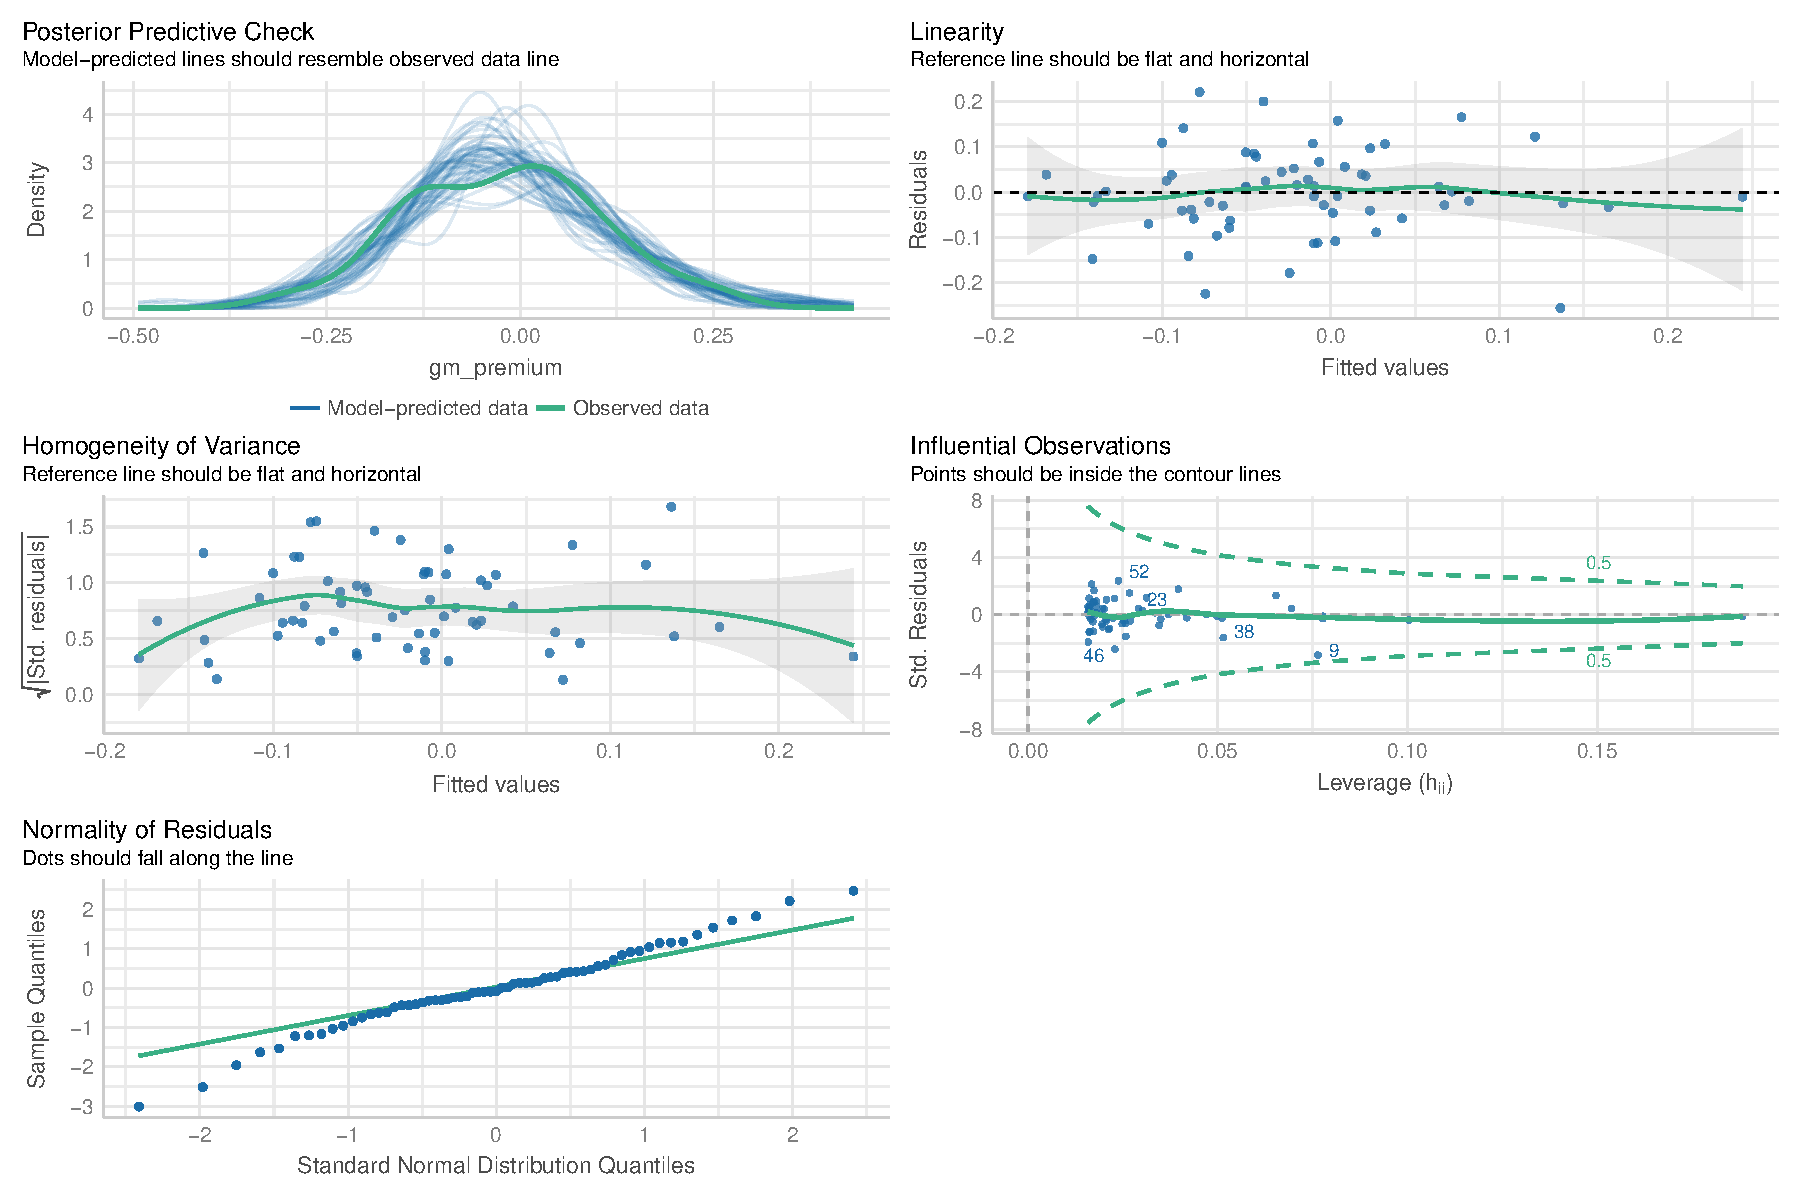
\includegraphics{capm_files/figure-latex/unnamed-chunk-14-1.pdf}
\caption{Regression Assumptions - GM Model}
\end{figure}

\newpage

\begin{figure}
\centering
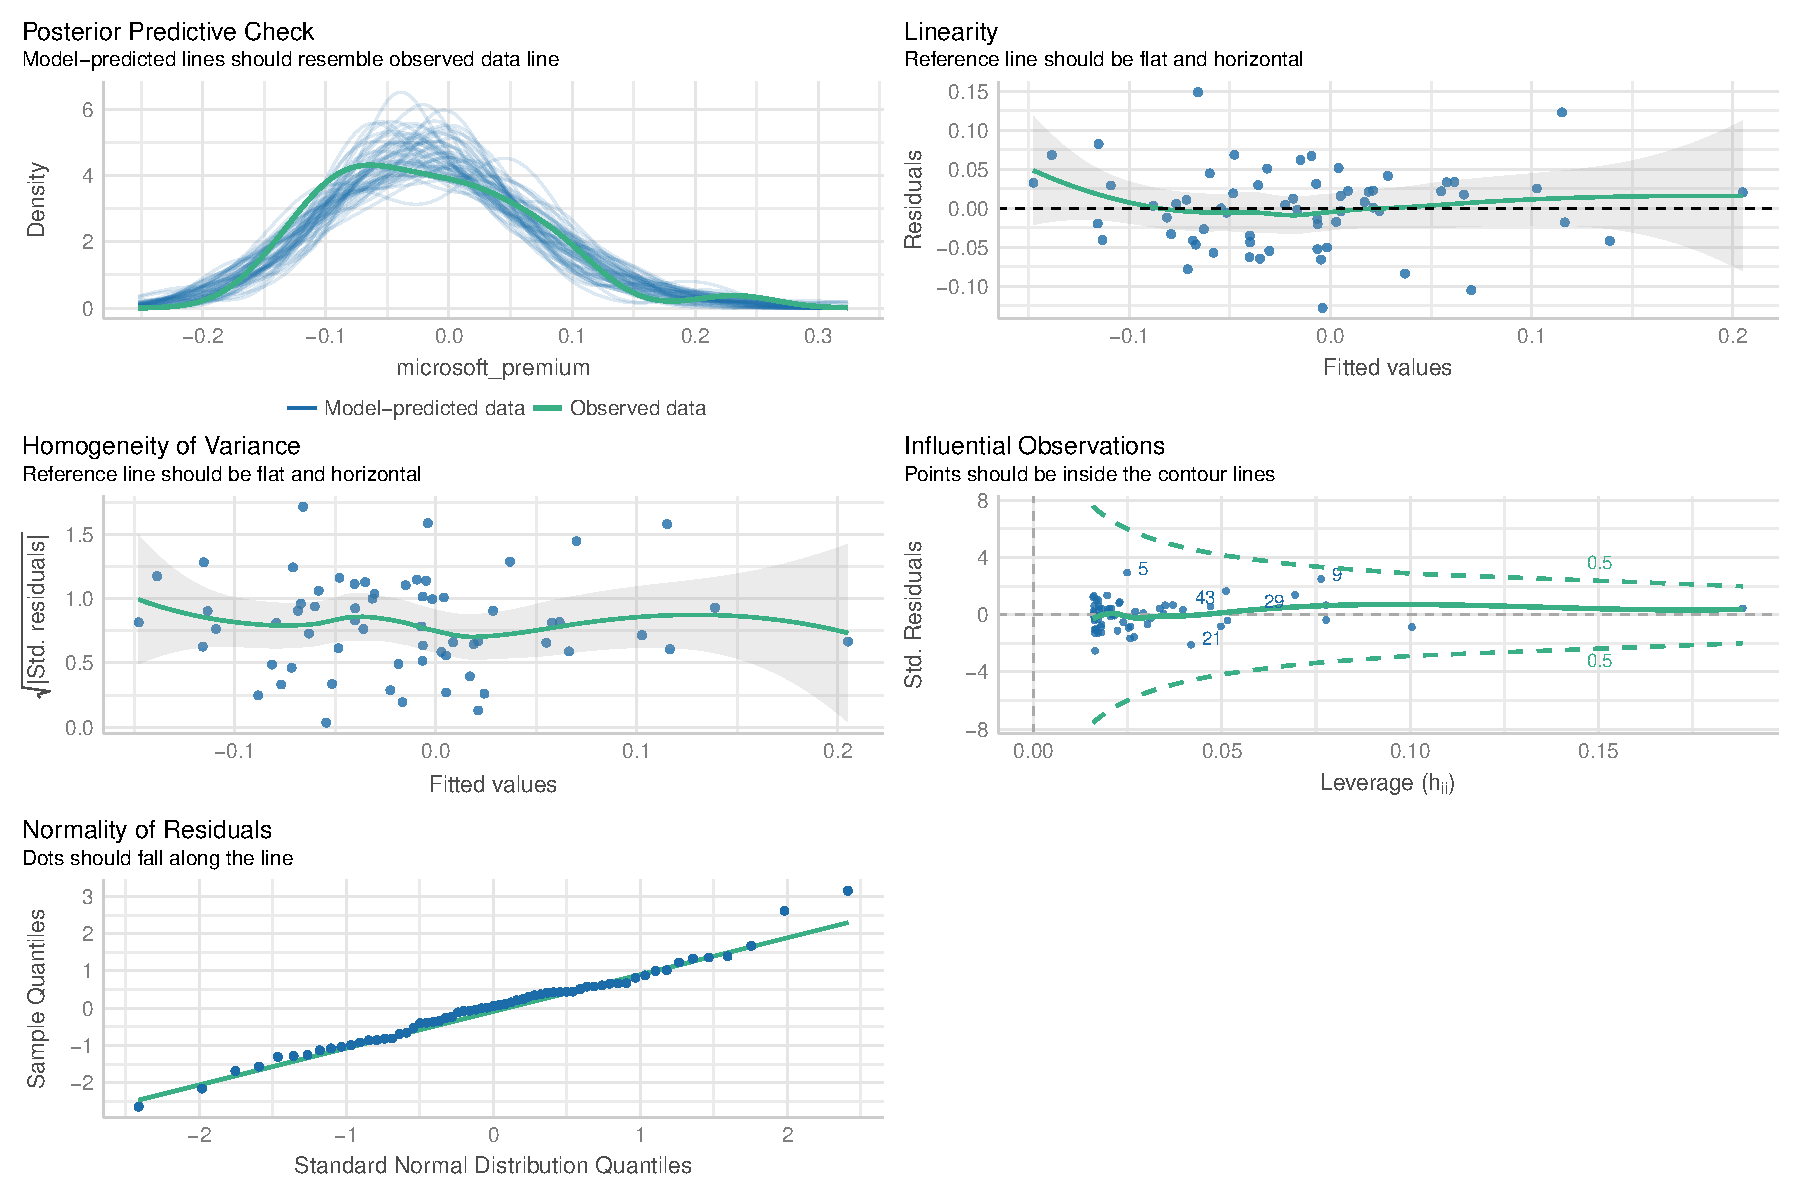
\includegraphics{capm_files/figure-latex/unnamed-chunk-15-1.pdf}
\caption{Regression Assumptions - Microsoft Model}
\end{figure}

\newpage

\end{landscape}

\hypertarget{conclusion}{%
\section{Conclusion}\label{conclusion}}

In this analysis, we estimated the \(\beta\) for GM and Microsoft stocks
using the CAPM. The results show that both stocks are as volatile as the
market portfolio. However, the analysis could suffer from omitted
variables bias.

\hypertarget{references}{%
\section{References}\label{references}}

Bodie, Z., Kane, A., Marcus, A.J. and Mohanty, P. (2018) Investments.
6th Edition, Tata McGraw-Hill Publishing Company, New Delhi.

\end{document}
